\documentclass[11pt]{article}
\usepackage{graphicx}
\usepackage{amssymb}
\usepackage{epstopdf}
\usepackage{amsfonts}
\usepackage{natbib}
\usepackage{subfigure}
\usepackage{pdfsync}
\usepackage{xspace}
\usepackage{color}
\usepackage{rotating}

%% some handy things for making bold math
\def\bm#1{\mathpalette\bmstyle{#1}}
\def\bmstyle#1#2{\mbox{\boldmath$#1#2$}}
\newcommand{\thh}{^\mathrm{th}}


%% Some pretty etc.'s, etc...
\newcommand{\cf}{{\em cf.}\xspace }
\newcommand{\eg}{{\em e.g.},\xspace }
\newcommand{\ie}{{\em i.e.},\xspace }
\newcommand{\etal}{{\em et al.}\ }
\newcommand{\etc}{{\em etc.}\@\xspace}



%% the page dimensions from TeXShop's default---very nice
\textwidth = 6.5 in
\textheight = 9 in
\oddsidemargin = 0.0 in
\evensidemargin = 0.0 in
\topmargin = 0.0 in
\headheight = 0.0 in
\headsep = 0.0 in
\parskip = 0.2in
\parindent = 0.0in


\title{Variation in Parentage-Based Tagging \\
and Coded-Wire  Tagging  Rates}
%\author{Eric C. Anderson\thanks{
%    Fisheries Ecology Division, 
%    Southwest Fisheries Science Center, 
%    110 Shaffer Road,
%    Santa Cruz, CA 95060}
%}
\begin{document}

\maketitle


\begin{abstract}
Realized rates of tagging are investigated for scenarios using parentage-based tagging (PBT)
and coded wire tags (CWT).  
Using CWTs the fraction of fish tagged can usually be accurately
estimated at the time of tagging/release, though there will be some variation in the realized
proportion of tagged versus untagged fish at the time of adult sampling.  In a PBT
scenario, the {\em expected} fraction of fish tagged at the time of tagging can be
estimated from the number of successfully-genotyped male-female spawner pairs that
contributed to the release group.  However, unless 100\% of the parents producing the release
group are successfully genotyped, the realized PBT tagging rate can differ from the
expected rate because different families produce different numbers of offspring that survive
at different rates to time of tagging.  Additional variation is possible due to differential
survival of family groups to the time of adult sampling.  These issues, as well as their
consequences for the variance in the estimated expanded number of recoveries, are explored
through simulation.  The results suggest that it is best to maintain a high ($>96\%$) fraction
of successfully genotyped parent pairs, especially when a high fraction ($\geq 75\%$) of the
release group is marked.

\end{abstract}


\tableofcontents

Our goal here is to develop a simple system of simulations to describe, explore, and understand
variation in the realized tagging rates achieved when using parentage-based tagging (PBT)
or coded-wire tags (CWTs) for hatchery-raised salmon.  Here we describe simulation routines
and the assumptions made in them for both CWTs and PBT.

\section{Tagging rates of CWTs}
Coded wire tags are typically deployed
when the fish are large enough to be tagged and to have their adipose fins clipped, frequently
just days before release.  In large hatchery programs, the tagging of release
groups is often undertaken with specialized tagging trailers that automate the tagging and marking
process and usually allow for a precise count of the number of fish tagged,
as well as the total number of fish in the release group.  Within a release group, the tags are
assumed to be randomly assigned to individual fish, so there is no association between the family
the fish came from and whether or not it carries a tag.  For these simulations, we will assume
that the CWT tagging rate, $p_\mathrm{cwt}$, is known without error at the time of release and that
the rate of tag shedding has been accounted for in it. 

Most CWT recaptures occur in adult fish.  Each tagged fish at the time of recovery can be
expanded by $1/p_\mathrm{cwt}$ into an estimate of the total number of impacts that the tag recovery represents.
Usually, $p_\mathrm{cwt}$ will provide a good estimate of the fraction of adult fish from the release group
that are tagged at the time of recovery, a proportion we will call the {\em realized} tagged
fraction, $\tilde{p}_\mathrm{cwt}$.  It should be clear that the realized
tagged fraction is the relevant quantity when expanding
tag recoveries of adult fish, but is typically not known.  
We will assume that tagged and untagged fish have the same rate of
survival so that adult fish can be regarded as a random sample from the fish in the release group (hence,
we are not modeling
effects of mark selective fisheries, etc.).
Although the sampling is technically without replacement, it is reasonable to model the sampling as
with replacement because so few adults survive from any given cohort.  For our simulations, if we consider the
$N_A$ adults that have survived from a release group tagged at rate $p_\mathrm{cwt}$  we will
model $\tilde{p}_\mathrm{cwt}$ as having a scaled binomial distribution:
$	\tilde{p}_\mathrm{cwt} \equiv X/N_A$ where 
\[
X \sim \mathrm{Binomial}(N_A, p_\mathrm{cwt}).
\]


\section{PBT}
Determining expected and realized PBT tagging rates proceeds in a different fashion.  In PBT, the
offspring of a set of male and female spawners are raised separately in the hatchery
as a single release group. Let us assume that there are $S$ male-female pairs of spawners
whose eggs are contributed to the release group.  PBT will work most
efficiently with 100\% tagging---in other words, when all the parents of a release group
are genotyped.  However, there may be some rate at which genotypes are not obtained for certain
individuals.  Currently,
genotype data from both parents is  required for PBT; however, with newer genotyping
systems, that can economically provide more genotypes per individual, it will be possible
to accurately perform assignments of offspring to single parents.  Regardless of the exact mechanism,
we can still focus on the tagging rate of families (the offspring of two distinct parents) in the hatchery: under current practices
a family is tagged if both parents are genotyped; allowing single-parent assignments a family would be
considered tagged if at least one parent was genotyped.  For our 
simulations, we will let $G$ families out of $S$ be tagged.
Under this assumption, the
fraction of families that are PBT-tagged is,
\[
f_\mathrm{pbt} = \frac{G}{S}.
\]   
This quantity will typically be used as an estimate of $p_\mathrm{pbt}$, the expected PBT tagging rate.

 
  
Depending on how much information about spawning is recorded at the hatchery, there are various
ways one can go about predicting $G$ or $G/S$. 
If cross information is recorded at the
hatchery, $G$ can be recorded directly from the mating records and the record of successful genotypes.
If cross information is not recorded, then $G/S$ can be predicted from the total proportion of males and 
females contributing to the release group that were successfully genotyped (see Section~\textcolor{red}{XX}).
In our simulations we will assume that $G$ is known because we are most interested in the effect of family
size;  however, if one were interested, it would be possible to add another hierarchy to the simulations in which,
although $G$ is fixed for the simulation,  $f_\mathrm{pbt}$ had to be estimated from the proportion of males
and females successfully genotyped.


The realized PBT tagging rate both at the juvenile stage, and later at the adult stage,
will vary from $f_\mathrm{pbt}$ because 1) different females produce different
numbers of eggs that survive at different rates to the time of release and 2) different families
will have different survival rates after release.  We let $p_\mathrm{pbt}$ be the fraction of juveniles
within the release group that are PBT-tagged.  This value is simulated by first assuming that each
family produces a negative-binomial distributed number of offspring with mean $\mu$ and 
overdispersion parameter $r$, (hence giving a variance of $\mu + \frac{\mu^2}{r}$), and then
assigning the parents of those families randomly to successfully- or unsucessfully-genotyped
categories.  Here, we assume a 1:1 mating scheme in our simulations.  Operationally, here
are the steps to simulating $p_\mathrm{pbt}$:
\begin{enumerate}
\item Set values of the parameters for the simulation: $S$, $G$, $\mu$, and $r$.
\item The number of offspring, $J_i$, produced by the $i\thh$ family is independently and identically simulated 
from a negative binomial distribution.  That is:
\[
P(J_i = k | \mu, r) = \frac{\Gamma(r + k)}{\Gamma(r)k!}\biggl(\frac{r}{r+\mu}\biggr)^r 
\biggl(\frac{\mu}{r+\mu}\biggr)^k
\] 
for $k = 1, 2, \ldots$ and $i = 1,\ldots, S$.  
\item $G$ of the $S$ families are randomly selected to have both parents successfully genotyped. The
indexes of these familes are recorded as the set
$\mathcal{B}$.  
\item The fraction of PBT-tagged juveniles in the release group is recorded as
\[
p_\mathrm{pbt} = \frac{\sum_{i\in\mathcal{B}} J_i}{\sum_{i=1}^S J_i}.
\]
\end{enumerate}
 

At the end of the above steps we have a simulated value of $p_\mathrm{pbt}$.  But now we
need to simulate the realized PBT-tagged fraction of adults, $\tilde{p}_\mathrm{pbt}$. 
This is somewhat more complicated than for CWTs, because both the occurrence of tagging (\ie successful genotyping)
and post-release rates of survival
are family-specific.  Our simulation scheme has a mechanism to introduce additional
variability in family-specific survival at this stage.  We assume that family-specific survival rate from release
stage to adulthood is independent of the number of individuals each family produced in the release
group (a reasonable assumption, as the selective forces in the wild are very different from those in the 
hatchery).    These are the steps we take to simulate $\tilde{p}_\mathrm{pbt}$, using
quantities that were simulated above:
\begin{enumerate}
\item Set the value of an additional parameter needed for this part of the simulation: $N_A$, the number
of adults from the release group present at the time of sampling/recovery, and $\alpha$,
a parameter that controls variation in survival rate among families. 
\item Let 
\[
Y = (Y_1,\ldots, Y_S) \sim \mathrm{Dirichlet}(\alpha, \ldots, \alpha)
\]
be a symmetrically-distributed Dirichlet random vector with $S$ components (one for each family).  Note that
$\sum_{i=1}^S Y_i =1$.  The value $Y_i$ represents the probability that a member of the $i\thh$ family group
will survive to adulthood.  As $\alpha \rightarrow \infty$, the vector $Y$ approaches a vector with
all components equal to $1/S$ (all individuals survive at the same rate, regardless of family).  As $\alpha
\rightarrow 0$, $Y$ will have all its mass on one $i$, suggesting that only a single family has individuals
that survive.
\item Simulate $W_i$, the number of individuals from family $i$
that survive to adulthood, from a multinomial distribution
with $N_A$ trials and cell probabilities $q_i = \frac{Y_i J_i}{\sum_{i=1}^S Y_i J_i}$:
\[
W = (W_1,\ldots, W_S) \sim \mathrm{Mult}_S(N_A, (q_1, \ldots, q_S))
\]
\item The realized PBT-tagging rate amongst adult fish is recorded as:
\[
\tilde{p}_\mathrm{pbt} = \frac{\sum_{i\in\mathcal{B}} W_i}{\sum_{i=1}^S W_i}.
\]
\end{enumerate}


\section{Consequences of tag rate variation on expanded estimates}
The above has been developed as if every fish in a release group could potentially be 
sampled in a fishery.  However, it is common that only a fraction $m$ of a release
group might be marked and thus have the chance to be sampled.  In such cases, the mark 
rate must be taken into account to form an expanded estimate of the
total number of release group fish represented by tag recoveries.  
The influence of the variance of the tagging rate  is dependent on the mark rate.
In particular, the relevant quantity is the rate at which adult fish in the release group are
both tagged and marked, where we use ``marked'' to mean that they are able to be sampled in the 
fishery (thus, with electronic tag detection this would mean that the fish carry a CWT, and
for visually-sampled fisheries, this means that the fish has an ad-clip).  

In applying PBT, typically all the members of a release group will be tagged by PBT, and then a random fraction $m$ of those
will receive marks.  In the simulations the number of tagged and marked fish in the fishery is found by randomly assigning each of the $\sum_{i\in\mathcal{B}} W_i$ tagged fish to the marked category, independently, with probability $m$.  All of these fish are assumed to be sampled
and then an expanded estimate $T_\mathrm{pbt}$ of the total number of release group fish in the fishery is found by multiplying that by 
the expansion factor $1/(mf_\mathrm{pbt})$.

In our simulations, we simulate the actual value of the mark and tag rates for CWTs in a similar fashion (by randomly
assigning coded wire tagged fish to marked and unmarked categories) by assuming
that a fraction $m$ of the tagged adult fish present in the fishery received marks.  This makes it easy to identify the additional variance in
PBT sampling due to variance in family size.  But it should be kept in mind that, in many release groups, an effort is made to tag
the marked component at a rate of 100\%.  All marked fish with CWTs are assumed to be sampled from the fishery
and the expanded estimate $T_\mathrm{cwt}$ is obtained for each replicate by multiplying the
number of recoveries by $1/(mp_\mathrm{cwt})$.

 
\section{Interpretation of parameters $r$ and $\alpha$}

The parameters $r$ and $\alpha$ are the two that directly affect variance in family size.  $r$ 
controls the variance in the number of juveniles from each family at the time of tagging.  It is meant
to reflect variation between females in fecundity and family-specific variation in smolt to adult survival.  
Given a mean number of juveniles, $\mu$, a good rule of thumb is that roughly $\frac{2}{3}$ 
of the variation will be contained
within the interval $\mu \pm \sqrt{\mu + \mu^2/r}$.  For example, if the average number of smolts produced
per family is 3000, then setting $r$ to 9 means that roughly $\frac{2}{3}$ of the families will have
between 2000 and 4000 juveniles in the release group.


The interpretation of $\alpha$ will perhaps be even less familiar to most, and it also might not
be transparent how one should contextualize the joint effect of $r$ and $\alpha$ on the distribution
of family sizes at the time of adult sampling.  To aid in interpretation of how much variance in
family size is conferred by the combination of $r$ and $\alpha$ in any scenario, I estimate the
effective size of the population for each scenario.  This is done by simulating the number of
gene copies per family, $C_1,\ldots,C_S$,
for a constant sized population from a multinomial distribution:
\[
(C_1,\ldots, C_S) \sim \mathrm{Mult}_S(2S, (q_1, \ldots, q_S))
\]
and then calculating the probability that two gene copies sampled from amongst those offspring gene copies
are identical by descent (IBD) as:
\[
P(\mathrm{IBD}) = \frac{1}{4}\sum_{i=1}^S \frac{C_i}{2S}\frac{C_i - 1}{2S - 1},
\]
derived as follows: $\frac{C_i}{2S}$ is the probability that the first gene copy is sampled from family $i$;
$\frac{C_i - 1}{2S - 1}$ is the probability that the second gene copy is sampled from family $i$; if those two
gene copies are to be IBD, then they must both be from the same parent (probability 1/2) and they must be copies of
the same gene within that parent (probability 1/2), which gives the term of 1/4.  
$P(\mathrm{IBD})$ is recorded for each replicate at a particular value of $S$, $r$, and $\alpha$, the average
of those values, $\widehat{P(\mathrm{IBD})}$, is taken and the effective number of breeders is estimated
by $N_b = [2\widehat{P(\mathrm{IBD})}]^{-1}$.   The effect of the parameters controlling
variance in family size can thus be interpreted as the ratio of the effective number of spawners to the 
actual number of spawners, $\frac{N_b}{2S}$.

\textcolor{red}{Only a few estimates of the ratio of effective number of breeders to the census number of breeders ($N_b/N$) in salmon
hatcheries are available.  \citet{Moyeretal2007} report estimates of between 0.76 and 0.84 for coho in two different 
Oregon hatcheries.  For Chinook, Mike Ackerman provided us }

\section{Simulations}
\subsection{Simulation 1}
We first present simulations at 6 different values of $S = 10, 25, 50, 100, 250, 1000$.  For each value of $S$,
we assume two different values for the number of $G$ out of $S$ that are genotyped: $G = \lfloor 0.8 S \rfloor$ and
$G = \lfloor 0.96 S \rfloor$ and 
we explore two different scenarios of variance in family size. The first is a scenario in which each family
produces a Poisson-distributed number of
juveniles at the release stage (equivalent to $\mu=3000$, and $r\rightarrow\infty$) and there is no
additional variance due to differential family 
survival, post-release (\ie $\alpha \rightarrow \infty$)---this is equivalent to reproduction in
a ``Wright-Fisher'' population. The second scenario, has
$\mu = 3000$, $r = 30$, and $\alpha = 1$, and produces an $N_b/(2S)$ ratio close to
0.5.  In all simulations, $A_F$, the number of adults remaining at the time of recovery, was set to 
be $10S$, or 5 times above replacement for the parents of the release group. One thousand replicate simulations were run for each of these 24 different combinations of simulation parameters. The resulting distribution of realized adult tagging
rates ($\tilde{p}_\mathrm{pbt}$ and $\tilde{p}_\mathrm{cwt}$)
are shown in Figures~\ref{fig:wf80}--\ref{fig:ne50-96}.


\begin{figure}
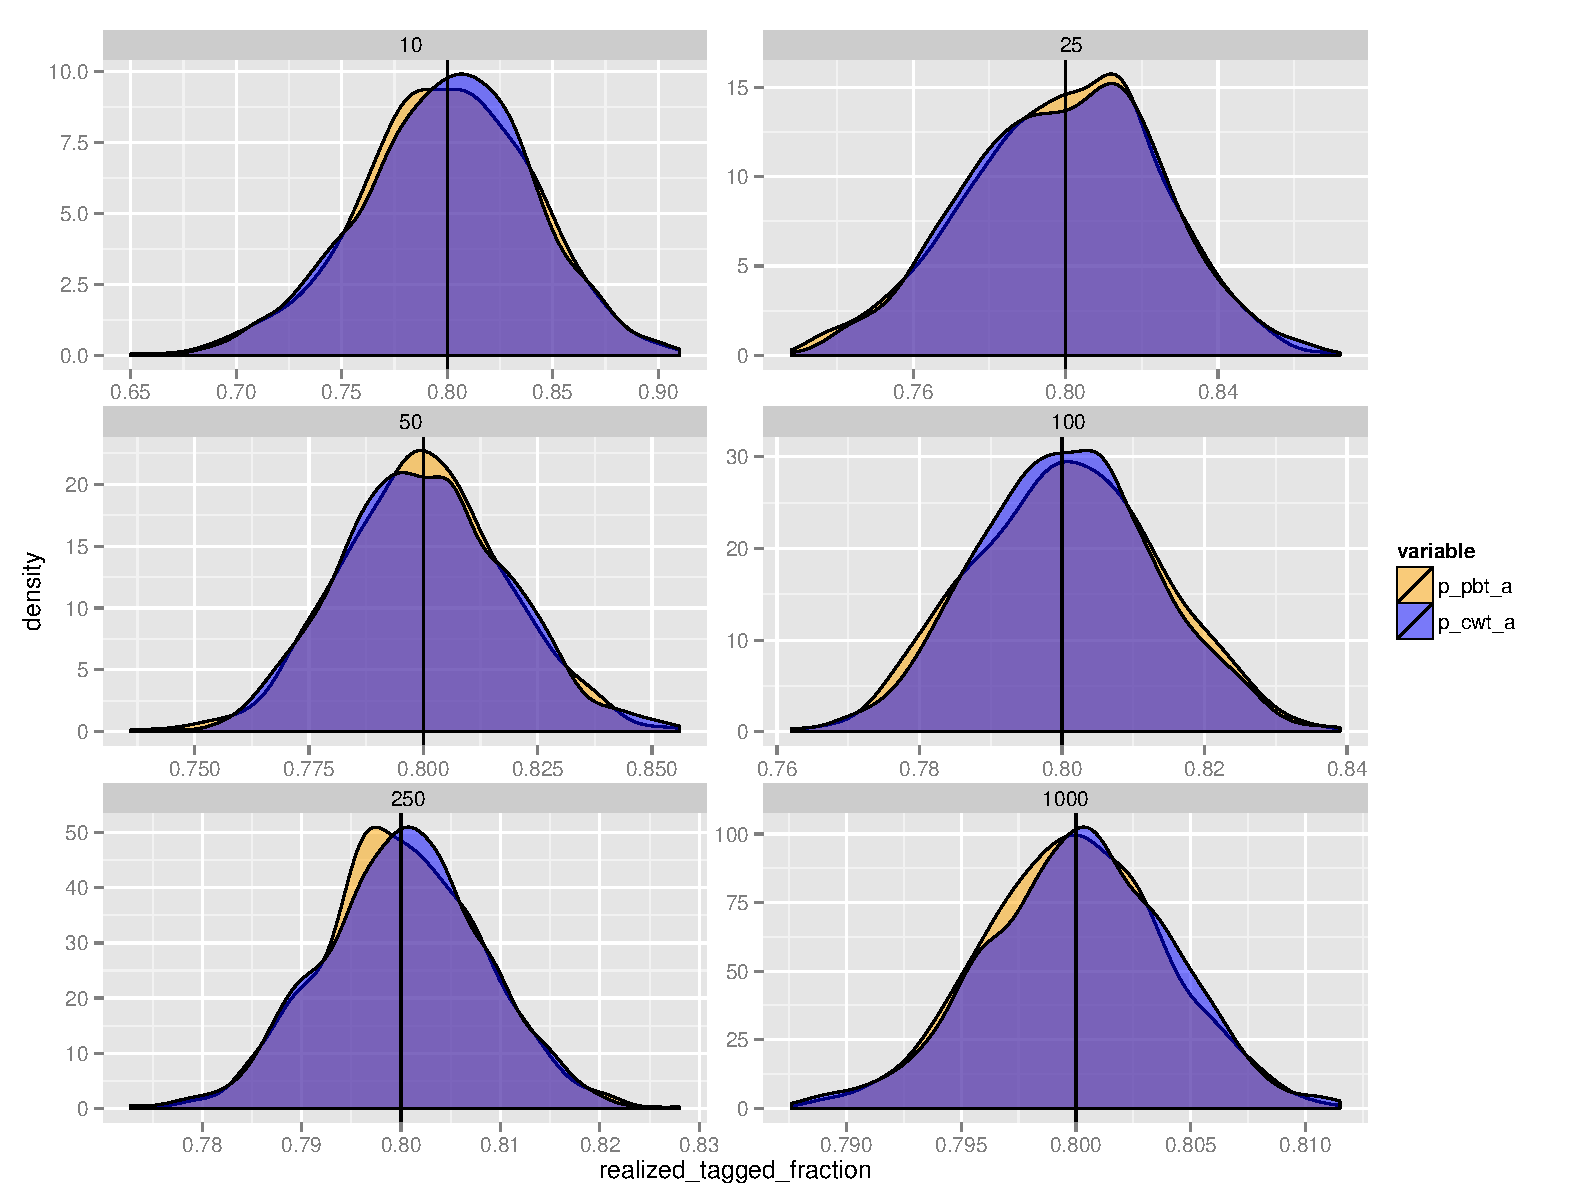
\includegraphics[width = \textwidth]{images/tag_fracts_80_WrightFisher.pdf}
\caption{Wright-Fisher variance in reproductive success. Expected tag rates of 80\%. Numbers
atop each panel give the number of families contributing to the release group. The black vertical line
gives the true fraction of families successfully genotyped or tagged at release by CWTs. Note that
scales differ between panels.}
\label{fig:wf80}
\end{figure}


\begin{figure}
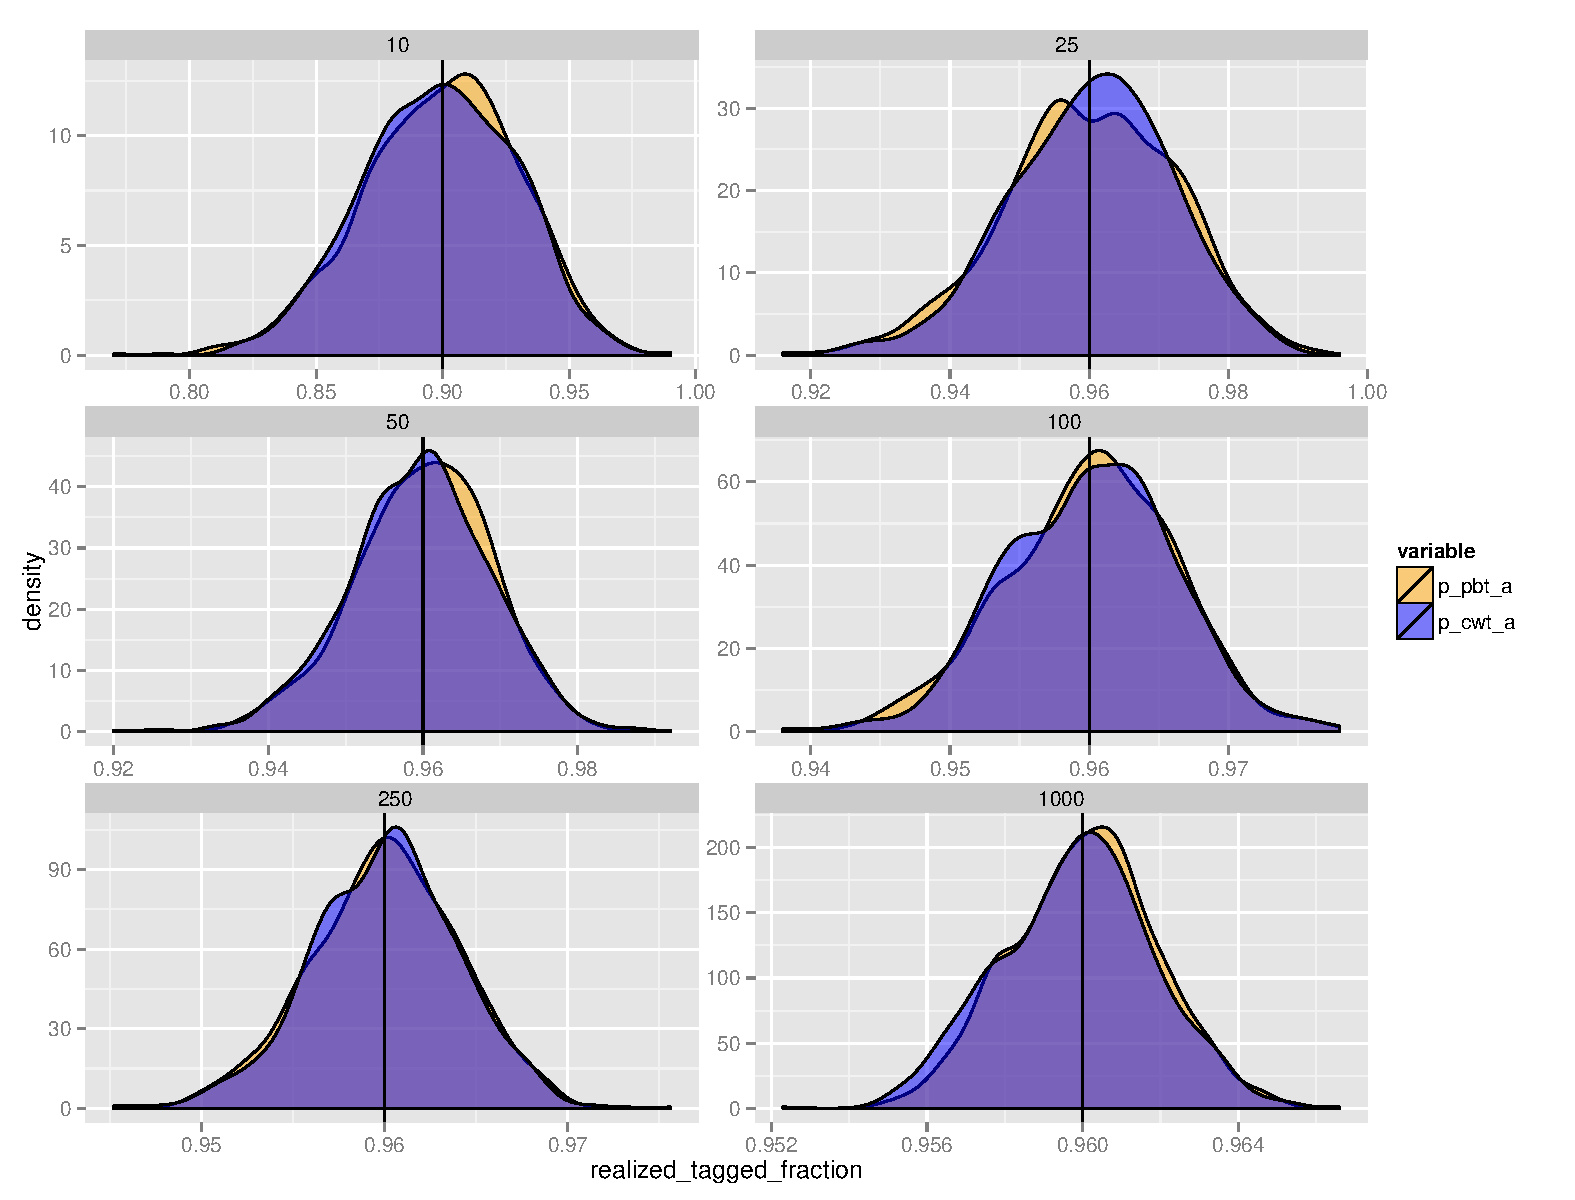
\includegraphics[width = \textwidth]{images/tag_fracts_96_WrightFisher.pdf}
\caption{Wright-Fisher variance in reproductive success. Expected tag rates of 96\%. For details
see caption of Figure~\protect\ref{fig:wf80}.}
\label{fig:wf96}
\end{figure}

\begin{figure}
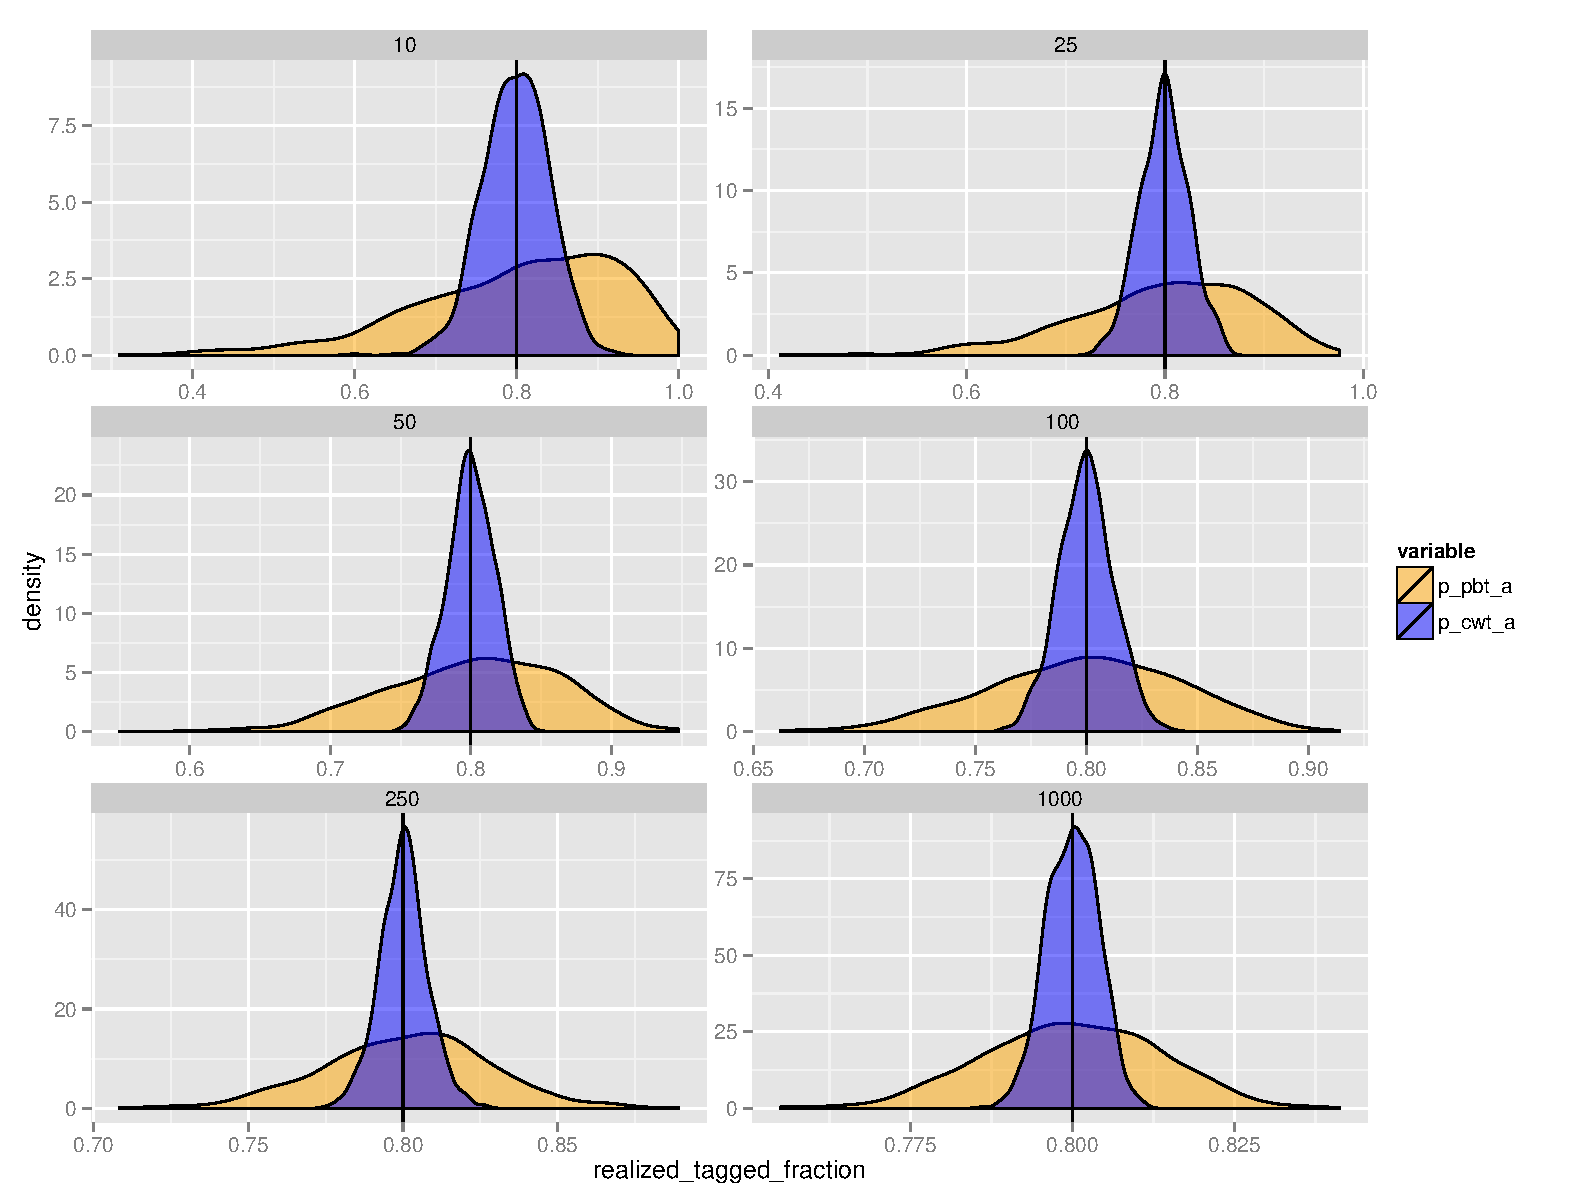
\includegraphics[width = \textwidth]{images/tag_fracts_80_Ne50.pdf}
\caption{Variance in reproductive success equivalent to an $N_e/N$ ratio of 0.5. Expected tag rates of 80\%. For details
see caption of Figure~\protect\ref{fig:wf80}.}
\label{fig:ne50-80}
\end{figure}

\begin{figure}
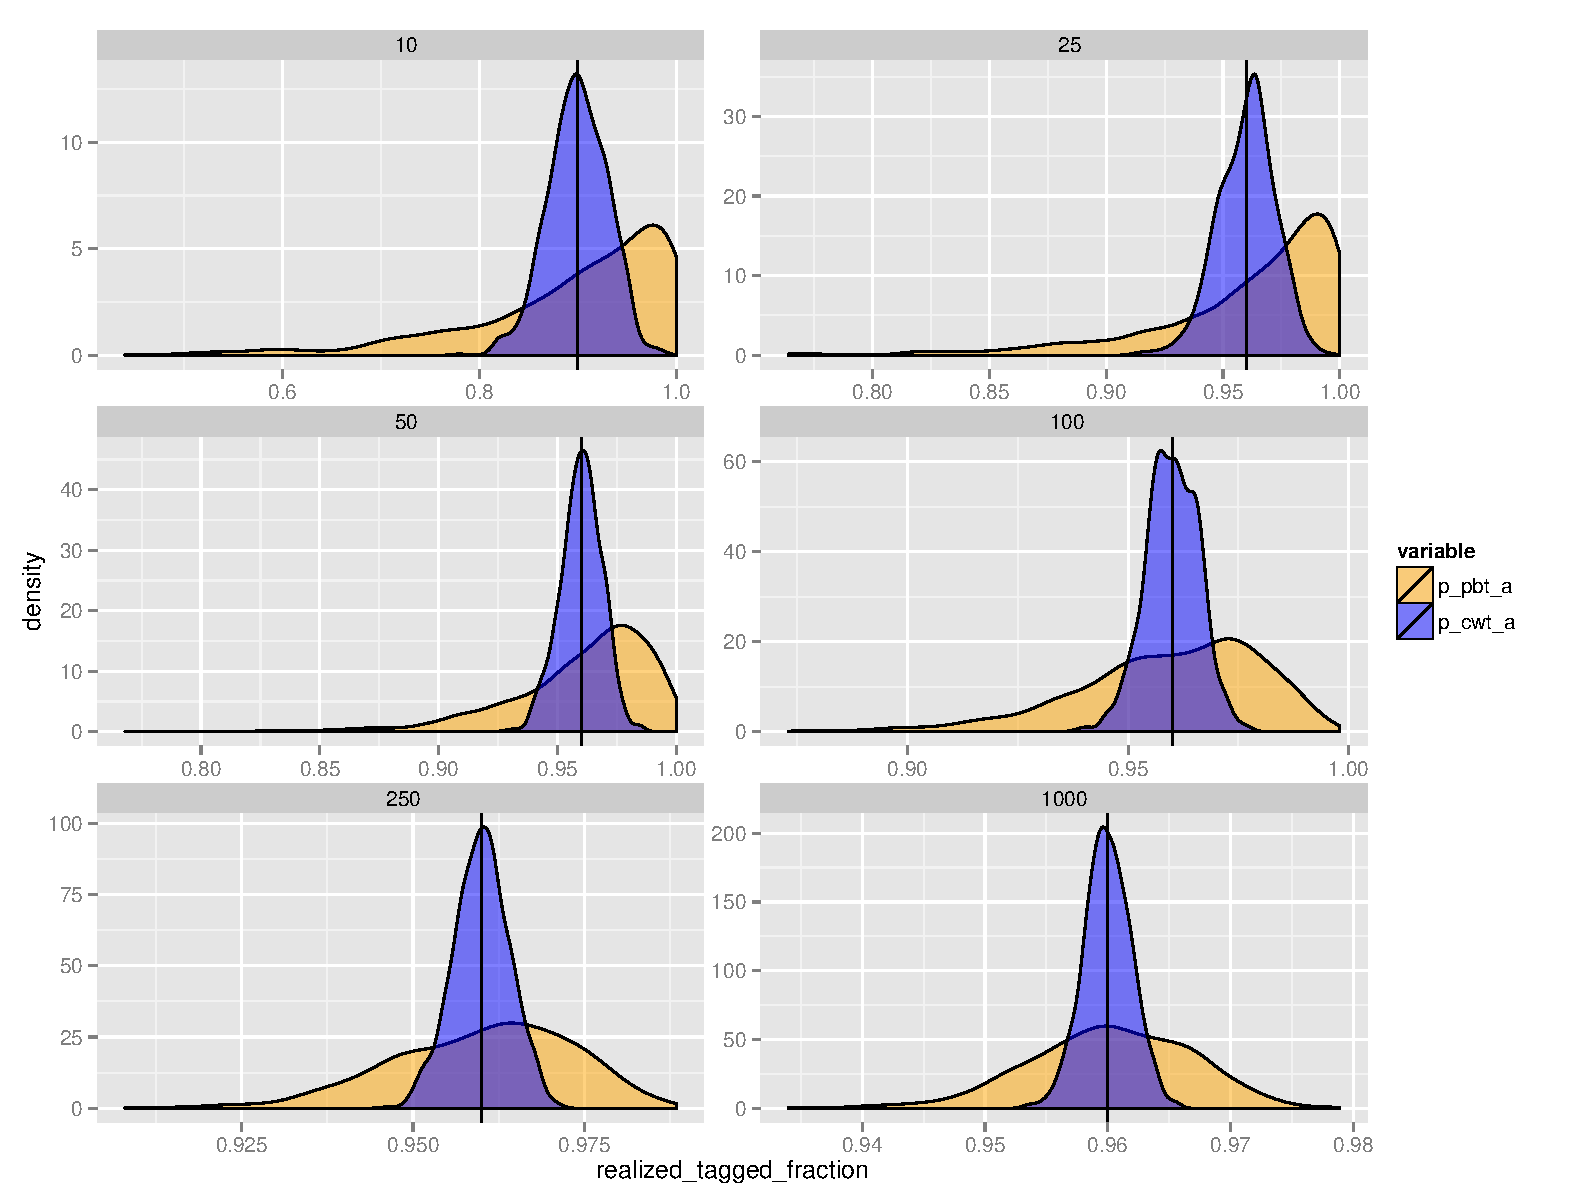
\includegraphics[width = \textwidth]{images/tag_fracts_96_Ne50.pdf}
\caption{Variance in reproductive success equivalent to an $N_e/N$ ratio of 0.5. Expected tag rates of 96\%. For details
see caption of Figure~\protect\ref{fig:wf80}.}
\label{fig:ne50-96}
\end{figure}

These simulations show that, if salmon populations reproduced in a Wright-Fisher fashion
(\ie Poisson distribution of family sizes), then the variation in
realized tagging rates for PBT would be commensurate with those for CWTs.  However, salmon populations
typically exhibit variance in reproductive success beyond that expected in a Wright-Fisher population, with
$N_b/(2S)$ ratios in  Oregon coho hatcheries reported to be between 0.76 and 0.84  \citet{Moyeretal2007}. 
 In such cases with overdispersed variance in reproductive success,
for release groups arising from few families ($<50$ families, for example),
there is an appreciable increase in the variance of the realized tagged fraction of adults using PBT when
not all of the parents were successfully genotyped.  However,
the consequence of this for different applications needs to be assessed. Accordingly a second set of simulations
was conducted in which the goal was to assess the effect on expanded numbers of fish. 

\subsection{Simulation~2}
250 replicate simulations were performed for every combination of the following set of values:
\begin{itemize}
\item $S \in \{10, 15, 20, 25, 30, 40, 50, 75, 100, 150, 200, 250, 400, 700, 1000\}$
\item $A_F = 5$
\item $G \in \{\lfloor a S\rfloor\}$ where $a \in \{0.80, 0.82, \ldots, 0.98, 1.00\}$, and with $p_\mathrm{cwt}$ set to the same
value as $\lfloor a S\rfloor$ in each case.
\item $\mu = 3000$, $r = 30$, and $\alpha \in \{0.5, 0.75, 1.0, 1.5, 2, 5, 10, 50\}$, as well as an additional scenario corresponding to
Wright-Fisher reproduction. 
\item $m \in \{0.25, 0.5, 0.75, 1.0\}$
\end{itemize}
For each scenario, it was assumed that there was a fishery in which 50 fish from the release group were caught and all fish
were sampled for marks, and fish with marks and tags (whether CWTs or PBT tags) were recovered and expanded back to
$T_\mathrm{cwt}$ and $T_\mathrm{pbt}$ according to the type of tag simulated.  The correct estimate of the expanded 
number of release group fish in the fishery is 50.  The number of tag recoveries expected in each simulation is
$50 m \lfloor a S \rfloor$.

Each of the different scenarios of family size variance produced a different ratio of $N_b/(2S)$ covering a broad range:
$(0.34, 0.43, 0.50, 0.59, 0.66, 0.81, 0.88, 0.95, 1.00)$, we summarize the results in terms of these $N_b/(2S)$ ratios
rather than in terms of $\alpha$, $\mu$, and $r$.

Figure~\ref{fig:all_sds} summarizes the standard deviation of the realized PBT and CWT tagging rates across all the scenarios.
\begin{sidewaysfigure}
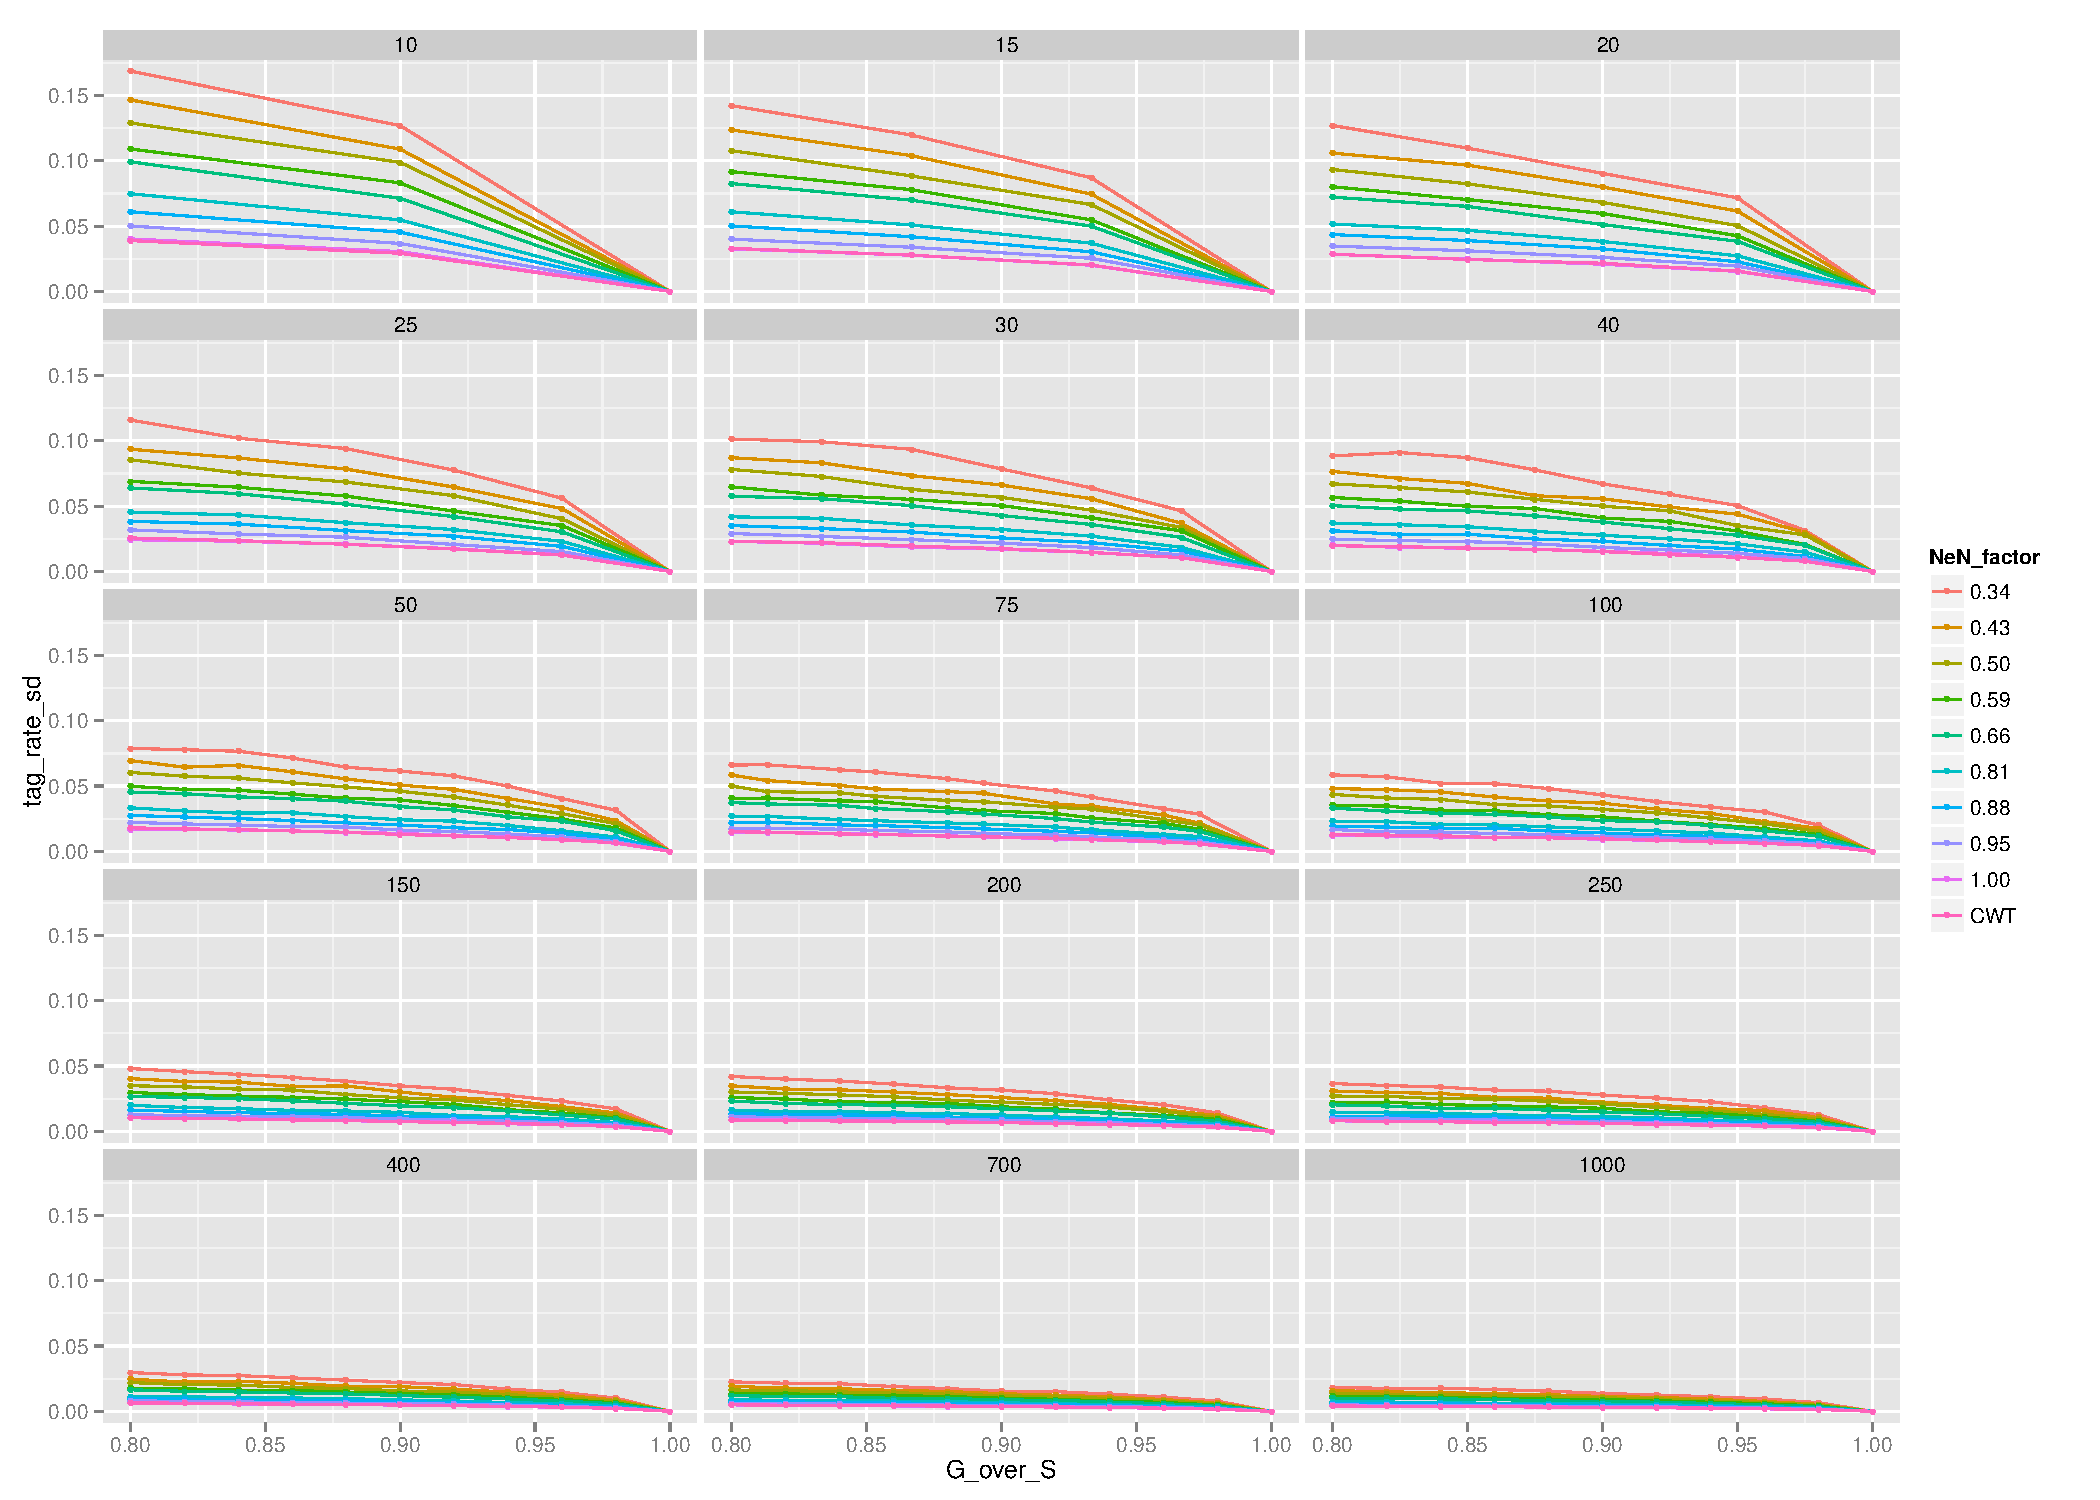
\includegraphics[width = .93\textwidth]{./images/tag_rate_standard_devs.pdf}
\caption{The standard deviation of the realized tagging rate $\tilde{p}_\mathrm{pbt}$ and $\tilde{p}_\mathrm{cwt}$.  $x$ axis shows the
expected tagged fraction $\lfloor G/S \rfloor$ in each simulation, $y$-axis gives the standard deviation over 1000 simulation replicates
for each point.  Colors denote different $N_b/(2S)$ ratios for PBT (or they denote CWT tagging in the bottom line in every panel).  Different
panels correspond to different numbers of $S$, as denote on the top of each panel.
\label{fig:all_sds}}
\end{sidewaysfigure}
It is clear that the variance of the realized PBT tagging rate is always higher than that of the CWT tagging rate, except in the case where
$N_b/(2S) = 1.0$, in which case the two are identical.  Standard deviation of $\tilde{p}_\mathrm{pbt}$ increases as $N_b/(2S)$ decreases and
as $S$ decreases.  


% m = 0.25
\begin{sidewaysfigure}
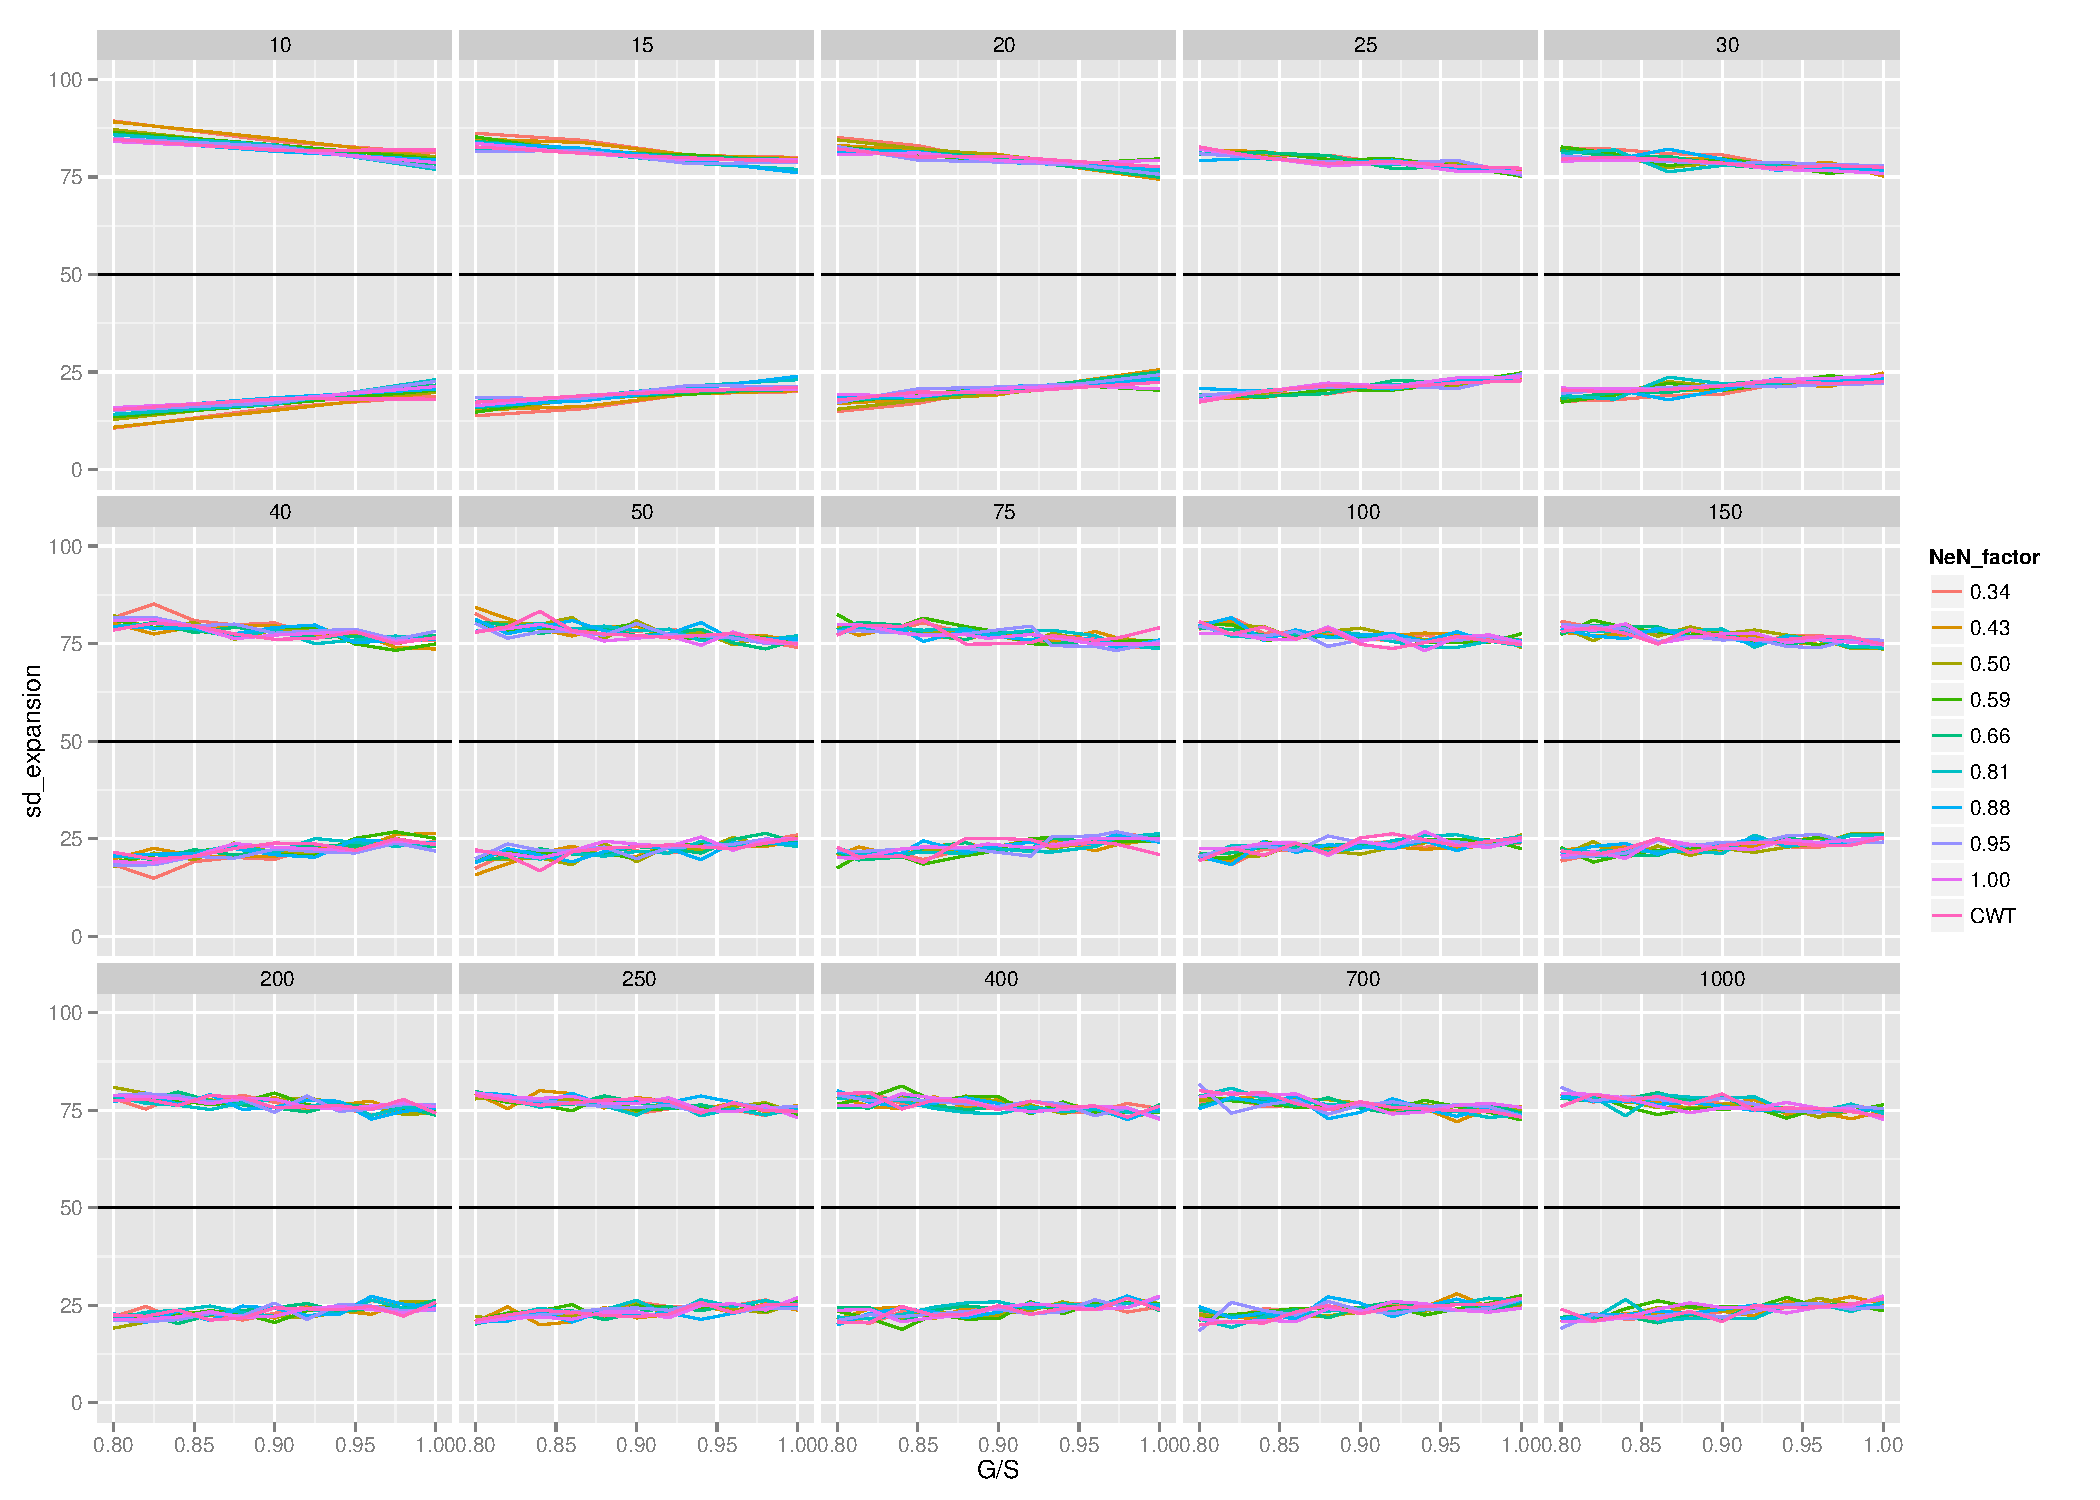
\includegraphics[width = .93\textwidth]{./images/sd_line_horns_m_0_25.pdf}
\caption{The uncertainty around expanded estimates using PBT or CWTs when $m = 0.25$.  $x$ axis shows the
expected tagged fraction $\lfloor G/S \rfloor$ in each simulation. Upon the $y$-axis is the number of fish from the
release group in the fishery (shown as the black horizontal line) and the mean estimate of that number from each different set of 
conditions plus or minus 2 standard deviations.  Thus, the vertical spread between lines of the same colour gives a representation
of the uncertainty in the estimate of the expanded number of fish. Colors denote different $N_b/(2S)$ ratios for PBT, or denote
the CWT estimate.  Different
panels correspond to different numbers of $S$, as denote on the top of each panel.
\label{fig:all_sds}}
\end{sidewaysfigure}


% m = 0.5
\begin{sidewaysfigure}
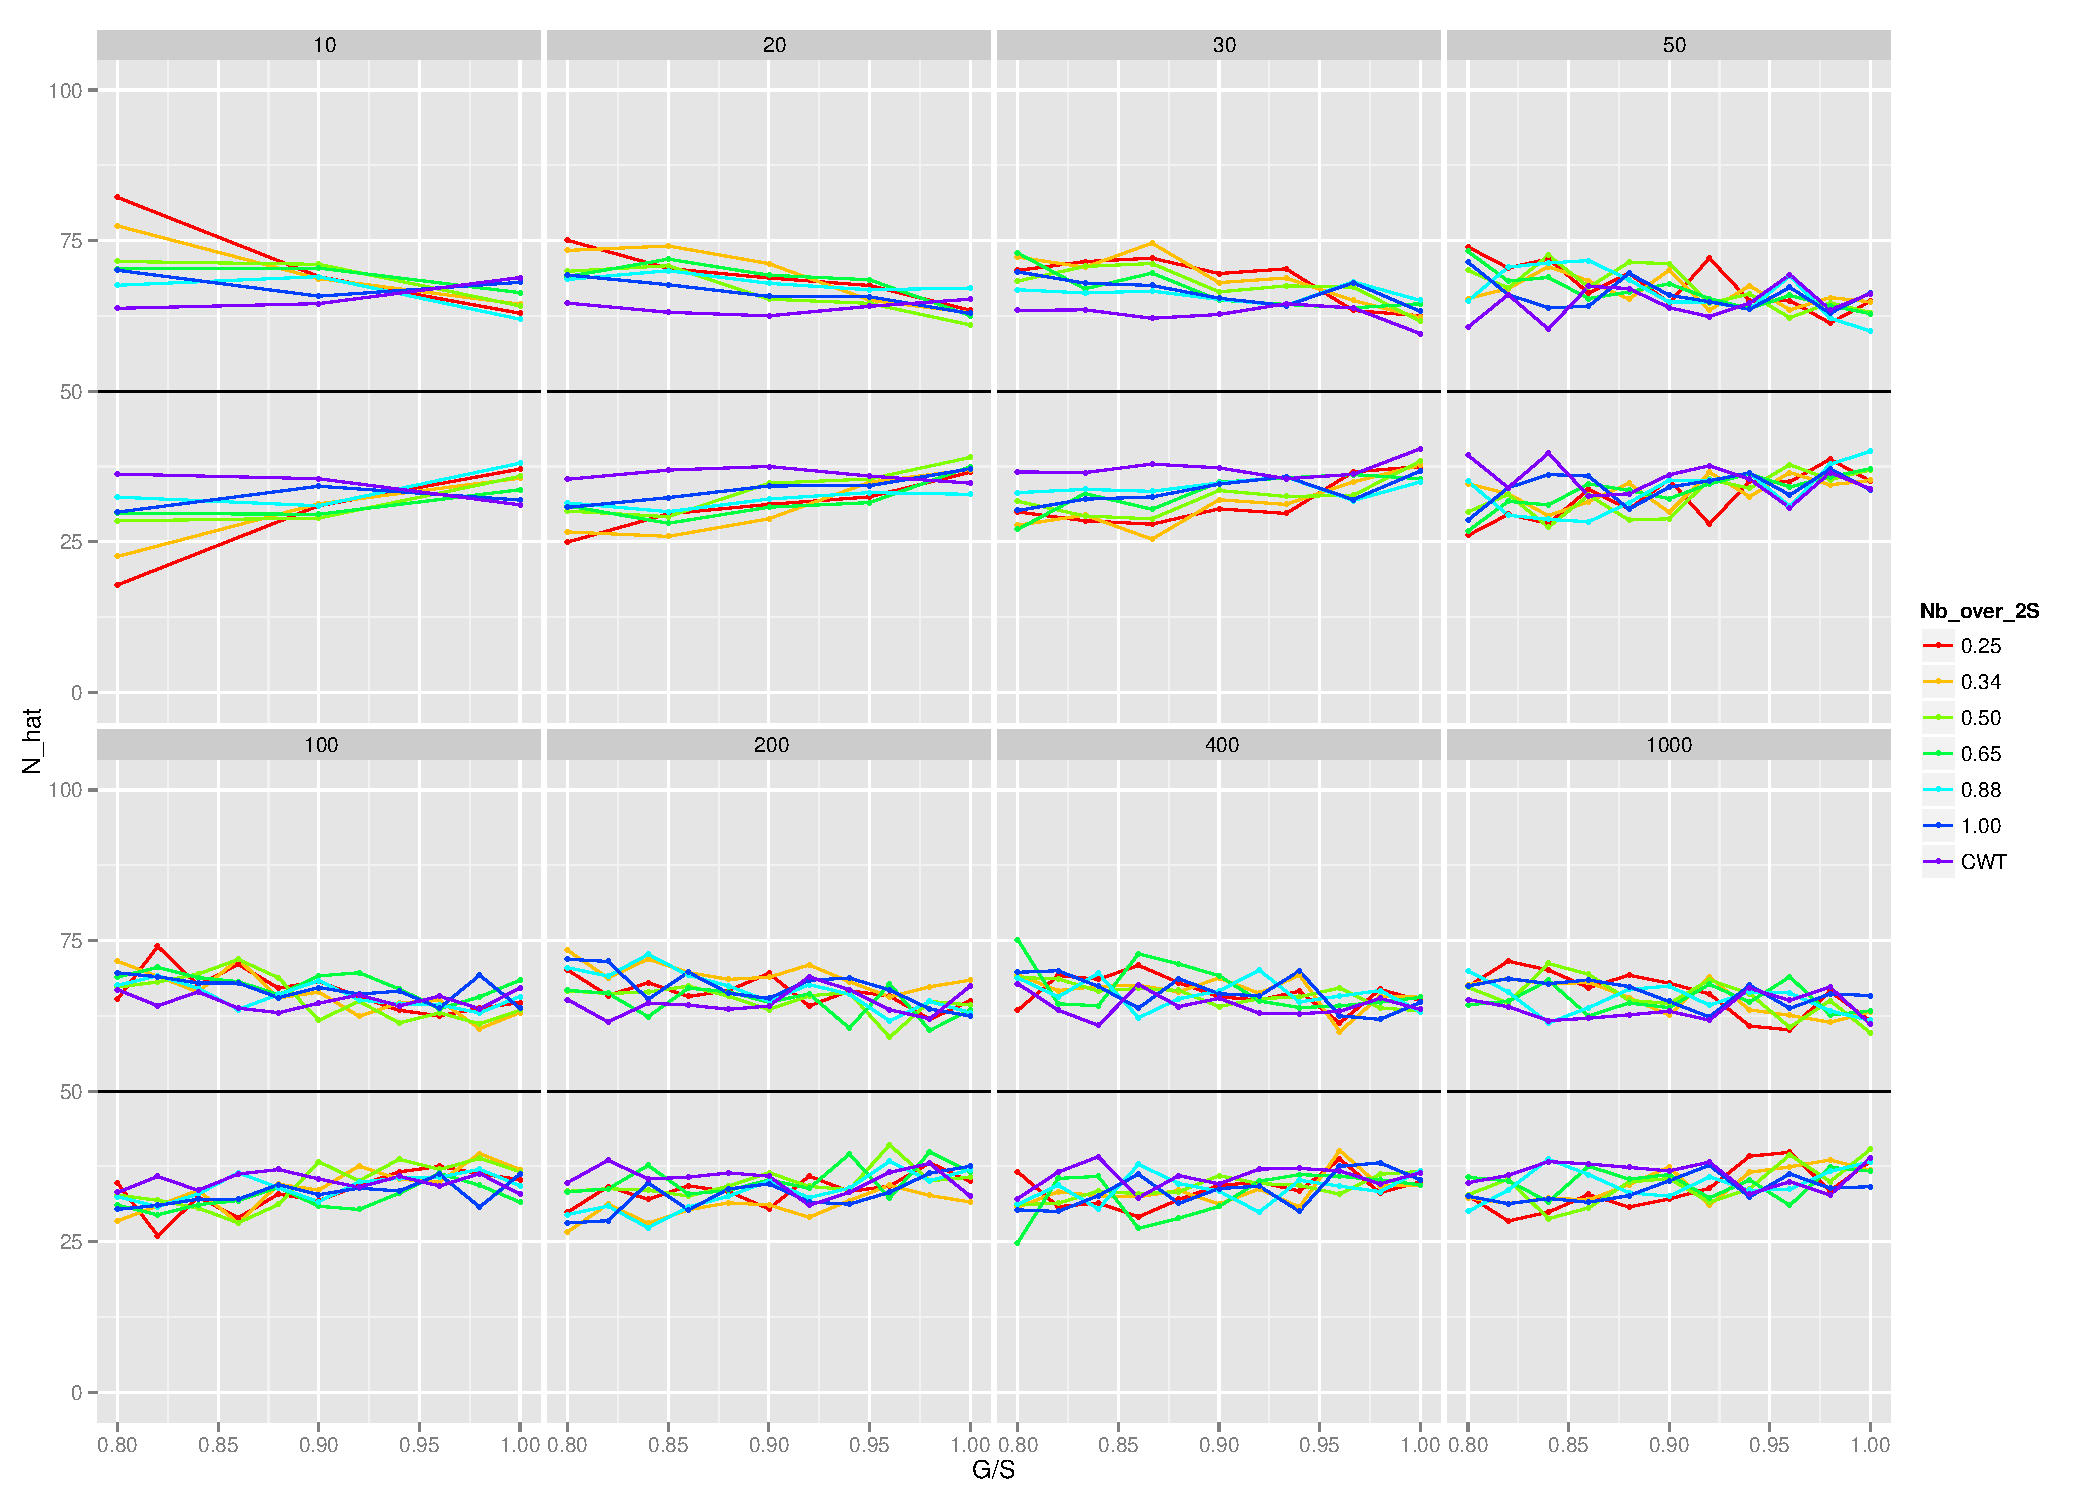
\includegraphics[width = .93\textwidth]{./images/sd_line_horns_m_0_5.pdf}
\caption{The uncertainty around expanded estimates using PBT or CWTs when $m = 0.5$.  $x$ axis shows the
expected tagged fraction $\lfloor G/S \rfloor$ in each simulation. Upon the $y$-axis is the number of fish from the
release group in the fishery (shown as the black horizontal line) and the mean estimate of that number from each different set of 
conditions plus or minus 2 standard deviations.  Thus, the vertical spread between lines of the same colour gives a representation
of the uncertainty in the estimate of the expanded number of fish. Colors denote different $N_b/(2S)$ ratios for PBT, or denote
the CWT estimate.  Different
panels correspond to different numbers of $S$, as denote on the top of each panel.
\label{fig:all_sds}}
\end{sidewaysfigure}

% m = 0.75
\begin{sidewaysfigure}
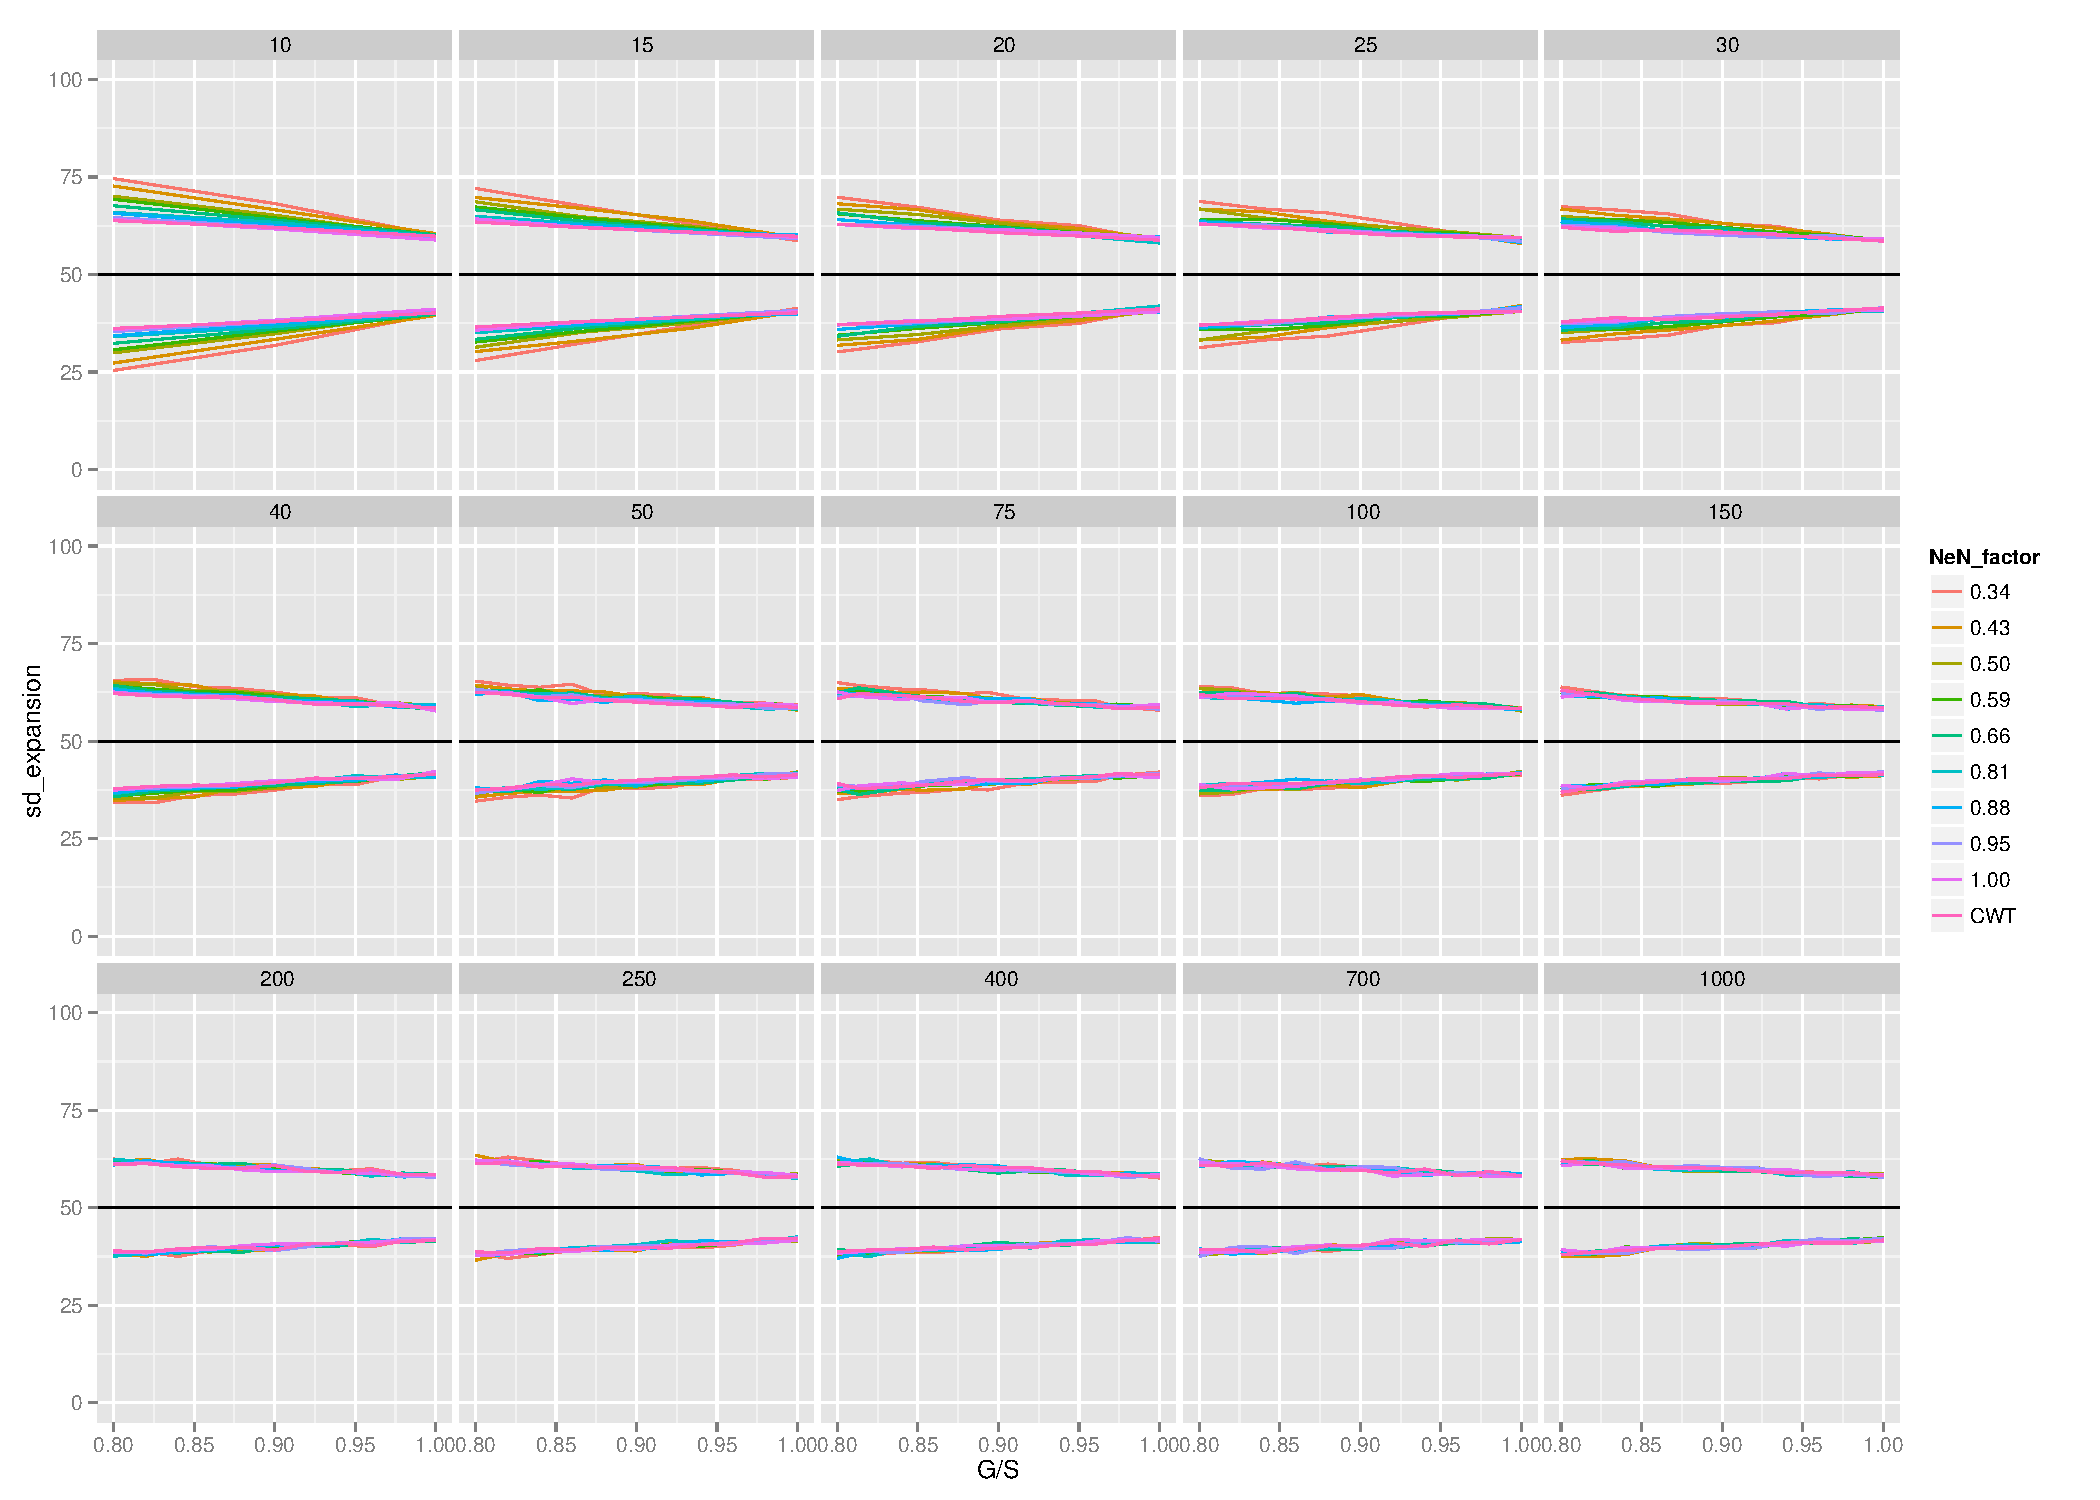
\includegraphics[width = .93\textwidth]{./images/sd_line_horns_m_0_75.pdf}
\caption{The uncertainty around expanded estimates using PBT or CWTs when $m = 0.75$.  $x$ axis shows the
expected tagged fraction $\lfloor G/S \rfloor$ in each simulation. Upon the $y$-axis is the number of fish from the
release group in the fishery (shown as the black horizontal line) and the mean estimate of that number from each different set of 
conditions plus or minus 2 standard deviations.  Thus, the vertical spread between lines of the same colour gives a representation
of the uncertainty in the estimate of the expanded number of fish. Colors denote different $N_b/(2S)$ ratios for PBT, or denote
the CWT estimate.  Different
panels correspond to different numbers of $S$, as denote on the top of each panel.
\label{fig:all_sds}}
\end{sidewaysfigure}



% m = 1.00
\begin{sidewaysfigure}
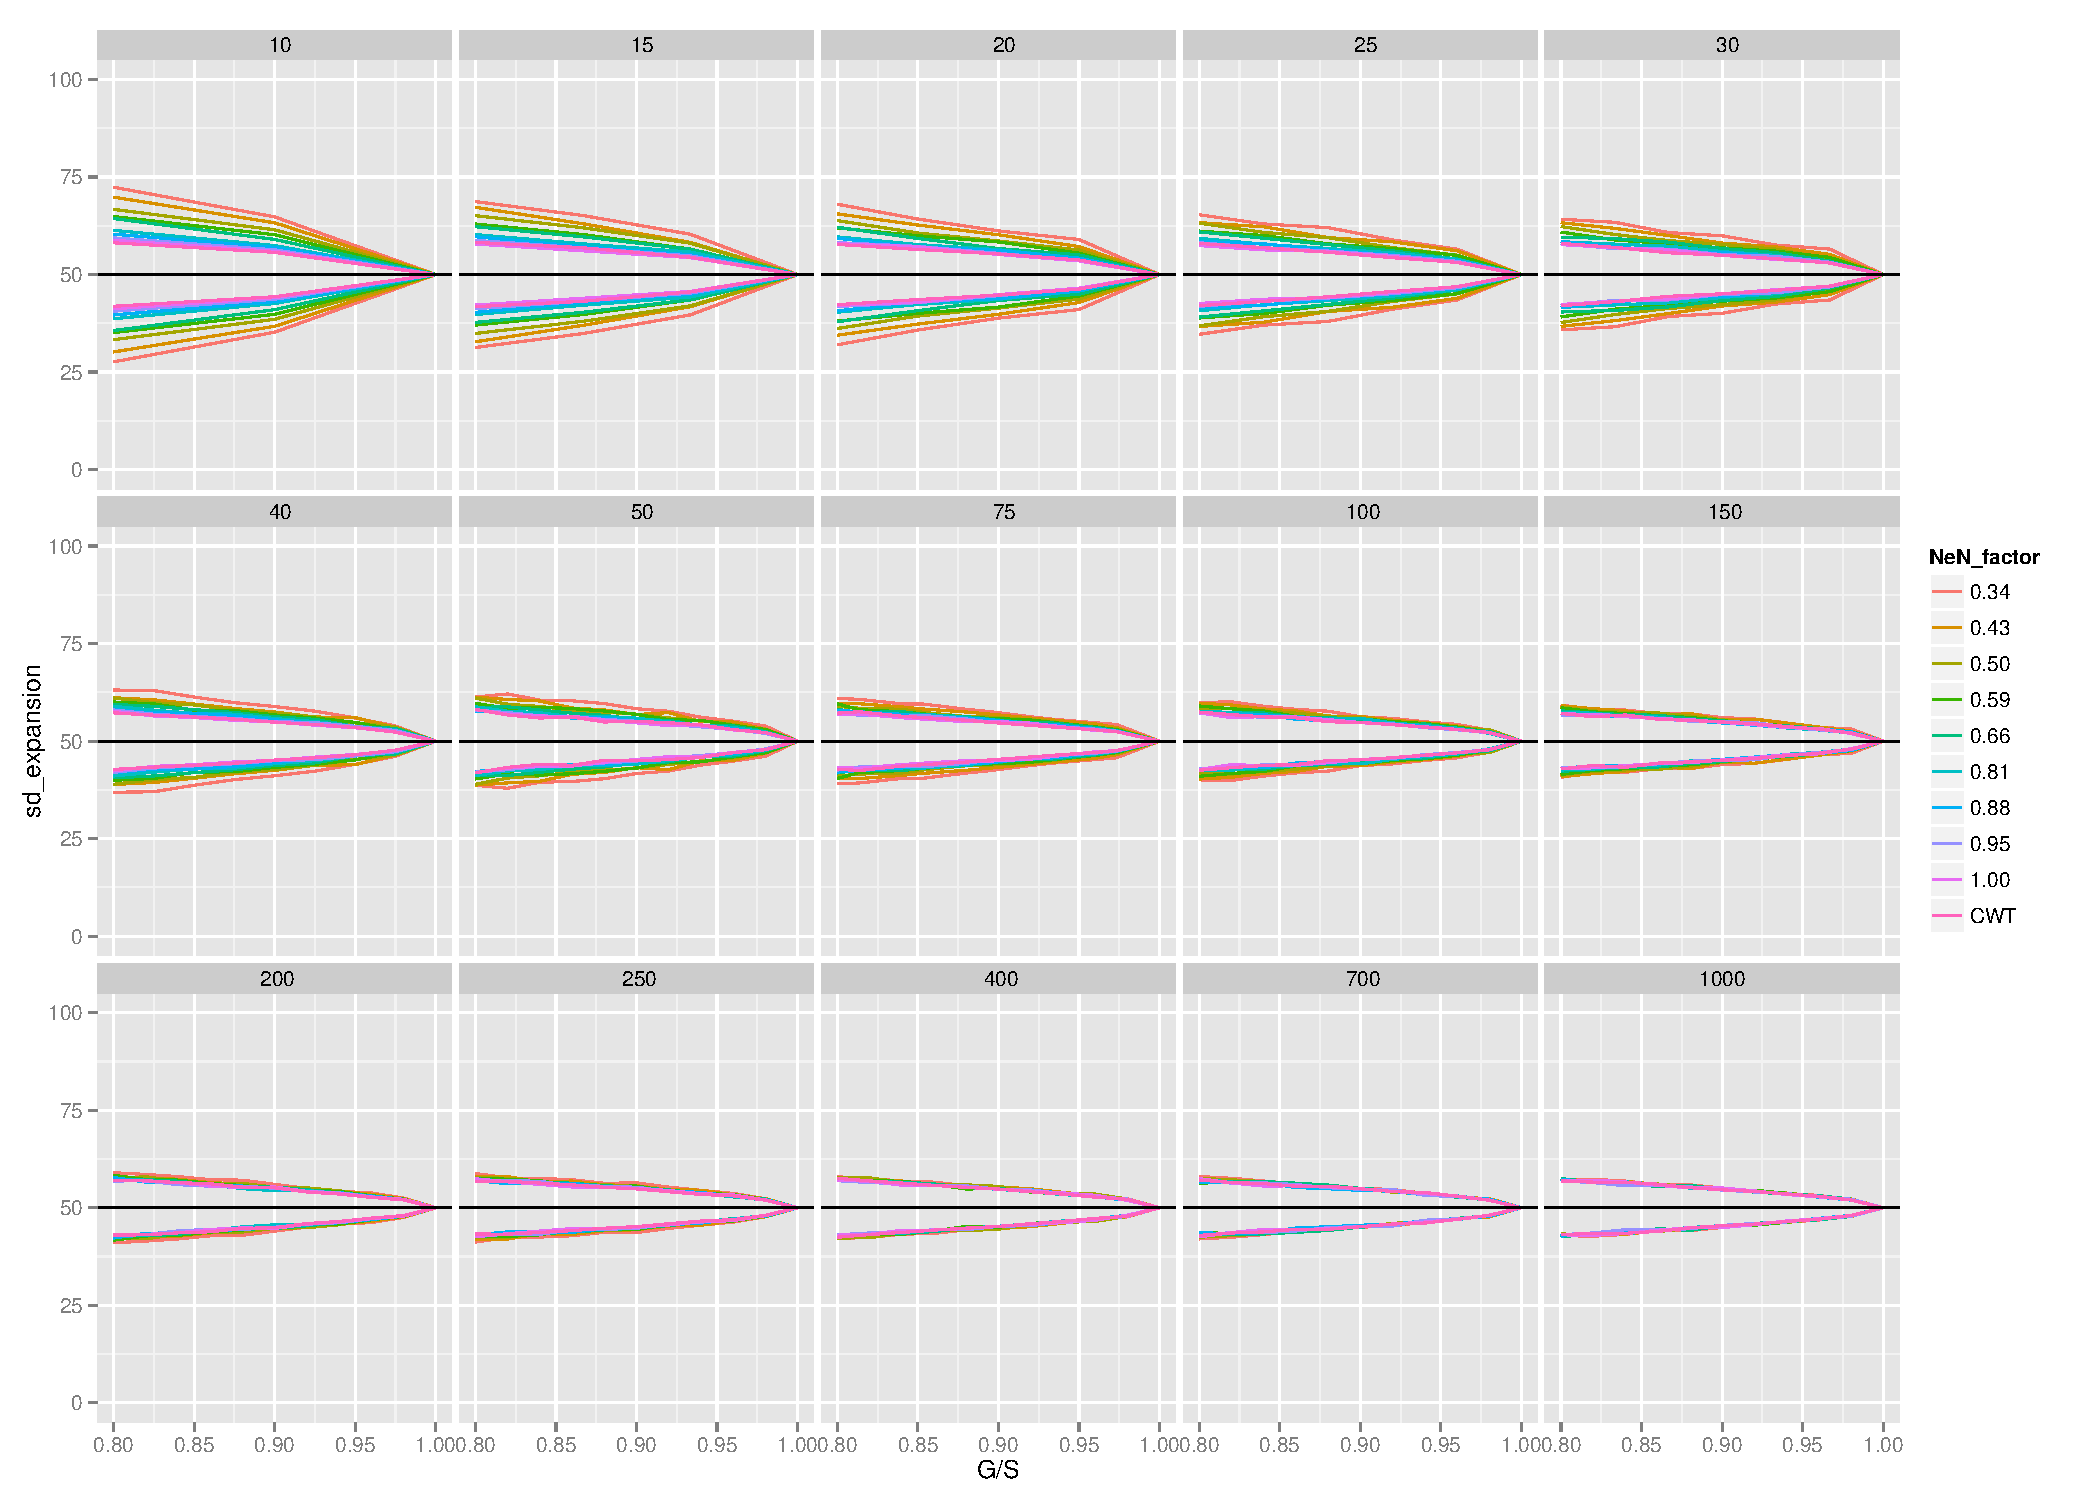
\includegraphics[width = .93\textwidth]{./images/sd_line_horns_m_1.pdf}
\caption{The uncertainty around expanded estimates using PBT or CWTs when $m = 1.00$.  $x$ axis shows the
expected tagged fraction $\lfloor G/S \rfloor$ in each simulation. Upon the $y$-axis is the number of fish from the
release group in the fishery (shown as the black horizontal line) and the mean estimate of that number from each different set of 
conditions plus or minus 2 standard deviations.  Thus, the vertical spread between lines of the same colour gives a representation
of the uncertainty in the estimate of the expanded number of fish. Colors denote different $N_b/(2S)$ ratios for PBT, or denote
the CWT estimate.  Different
panels correspond to different numbers of $S$, as denote on the top of each panel.
\label{fig:all_sds}}
\end{sidewaysfigure}


Need to describe the results\ldots.

Note that if the fishery is not sampled for marks at 100\% then that would need to be incorporated too, but clearly can be.


\section{Effective size of hatchery populations}

Would like to include a short analysis of Chinook data from Idaho showing $N_b/(2S)$ ratios of about 0.34 to 0.5.

\section{Actual sizes of release groups}
To know how much of an issue this is going to be we can look at the sizes of all the different
CWT-ed, chinook release groups since 2000.  For this analysis, I have assumed that if each release group
were to be tagged via PBT that it arose from spawnings at the hatchery in which the number of male
and female parents is equal and that each female produces 3000 offspring that survive to the release stage.

The results are in Table~\ref{tab:relsummary},
%%%%%%%%%%%%%%
\begin{table}
\caption{Summary of tagged chinook releases since brood year 2000 across all agencies.
The No.~releases column gives the number of families that would have been required to
create both the tagged and untagged components of the release group if number of male and female parents were equal and each female
averaged 3,000 smolts surviving to the release stage. The column No.~smolts gives the total number of smolts produced since 2000
in releases requiring number of familes in the range as given in No.~famimiles.  The column No.~releases gives the number of 
actual release groups in each No.~families category. \label{tab:relsummary}}
\begin{center}
\begin{tabular}{rrrrrr}
\hline\hline
No.~families  &  No.~smolts~released  &  No.~releases  &  \% of all smolts  &  \% of all releases \\ \hline
0--10  &   73,629,227  &  5,138  &  2.40  &  33.72\\
10--25  &  153,197,630  &  3,035  &  4.99  &  19.92\\
25--50  &  248,382,387  &  2,379  &  8.08  &  15.62\\
50--100  &  463,816,013  &  2,177  &  15.10  &  14.29\\
100--250  &  799,348,868  &  1,758  &  26.02  &  11.54\\
250--500  &  443,236,057  &    454  &  14.43  &  2.98\\
500--1,000  &  383,866,505  &    186  &  12.50  &  1.22\\
1,000--10,000  &  506,683,703  &    105  &  16.49  &  0.69\\\hline
\end{tabular}
\end{center}
\end{table}
%%%%%%%%%%%%%%%
which clearly show that a large fraction of all releases are very small (requiring less than 25 parents to produce it).
It is not clear to me why there are so many small release groups. With a tag recovery rate
of 2 in 1,000, it isn't clear that much is to be gained from releases of 30,000 fish taken on their own, especially if the
tagging rate is around 20\% and fish are recovered in highly stratified settings.  but if managers require all of these very small release
groups, this could present a challenge to PBT, and definitely warrants further discussion.





\bibliography{../bibstuff/pbtfeas}
\bibliographystyle{mychicago}
 \end{document}
